\section{Combined decomposition with the analytic recurrence}
\label{sec:notes-analytic-results}
The initial analytic-enabled comparison measures the added recurrence while preserving the existing learned models. It contains 16 rational-kinematics polygon requests, two fully symbolic two-point requests, 12 independent bubble products covering loop orders two through thirteen, eight nonplanar two-loop requests, and three further compatibility requests. Appendix~\ref{app:notes-analytic-inputs} specifies the denominators, targets, and parameter choices. Each method starts in a fresh process, and three repetitions rotate the method order on the same worker.

All four methods use the same independent-block factorization and share identical blocks within a request. The native control receives the same prepared master indices and uses the existing exact block formulas, but it generates native IBP equations for the newly supported one-loop blocks. The exact fixed control uses the new recurrence and disables learned choices. The preceding application runs unchanged with its earlier master-index cache. Its timer includes discovery and a second check when that cache lacks a structure. The matched native control receives the new prepared indices, which separates the recurrence benefit from this cache extension. Thus the native comparison measures the combined analytic and learned change, while the exact fixed comparison isolates the current learned contribution.

\begin{table}[!htbp]\centering\small
\caption{Complete decomposition times, summed over per-request medians. Speedup is native-control time divided by combined time. The last column is combined time divided by exact fixed-control time. Ratios below one in that column favor learned selection. Only requests verified in all three repetitions enter a paired sum.}
\label{tab:notes-analytic-results}
\begin{tabular}{@{}lrrrrr@{}}\toprule
Collection & $N$ & Combined (s) & Native (s) & Speedup & ML/fixed\\\midrule
Scalar one-loop polygons & 18 & 14.815 & 20.862 & 1.41 & 0.991 \\
Independent products & 12 & 4.524 & 9.522 & 2.10 & 1.063 \\
Coupled ML cases & 8 & 43.037 & 71.455 & 1.66 & 0.936 \\
Other compatibility cases & 3 & 2.890 & 2.918 & 1.01 & 0.978 \\
All requests & 41 & 65.266 & 104.757 & 1.61 & 0.958 \\
\bottomrule\end{tabular}
\end{table}

The combined application completes 41 of 41 requests in all three repetitions. The native, exact fixed, and preceding applications complete 41, 41, and 41 requests, respectively. Including every requested first attempt, the combined application takes 68.401 seconds. Independent reference and master-index preparation takes 357.770 seconds and remains outside the supplied-basis timer.

Against the actual preceding application, the combined method takes 65.266 seconds, compared with 103.134 seconds on 41 matched requests, giving a speedup of 1.58. This comparison includes each application's own preparation and recovery inside its timer.

Across all repetitions, the combined application makes 30 native calls, compared with 120 for the matched native control. The exact fixed control makes 48 calls, including 18 unsuccessful attempts before recovery. The combined method has 0 failed native calls. Thus the recurrence removes native work in its domain, and the retained learned selector avoids the failed sparse attempts observed with the fixed choice.

For the requests that use the new recurrence, the combined application uses 36.4\% less time than the matched native control. The time ratio is 0.636, with repetition interval $[0.608,0.748]$.

For the requests that use the new recurrence, the combined application uses 0.7\% more time than the exact fixed control. The time ratio is 1.007, with repetition interval $[0.787,1.208]$. This interval includes equal times, so this comparison does not resolve a saving beyond the observed repetition variation.

For the coupled nonplanar requests, the combined application uses 39.8\% less time than the matched native control. The time ratio is 0.602, with repetition interval $[0.568,0.635]$.

For the coupled nonplanar requests, the combined application uses 6.4\% less time than the exact fixed control. The time ratio is 0.936, with repetition interval $[0.873,0.988]$.

For all matched requests, the combined application uses 37.7\% less time than the matched native control. The time ratio is 0.623, with repetition interval $[0.599,0.662]$.

For all matched requests, the combined application uses 4.2\% less time than the exact fixed control. The time ratio is 0.958, with repetition interval $[0.869,1.017]$. This interval includes equal times, so this comparison does not resolve a saving beyond the observed repetition variation.

\begin{figure}[!htbp]\centering
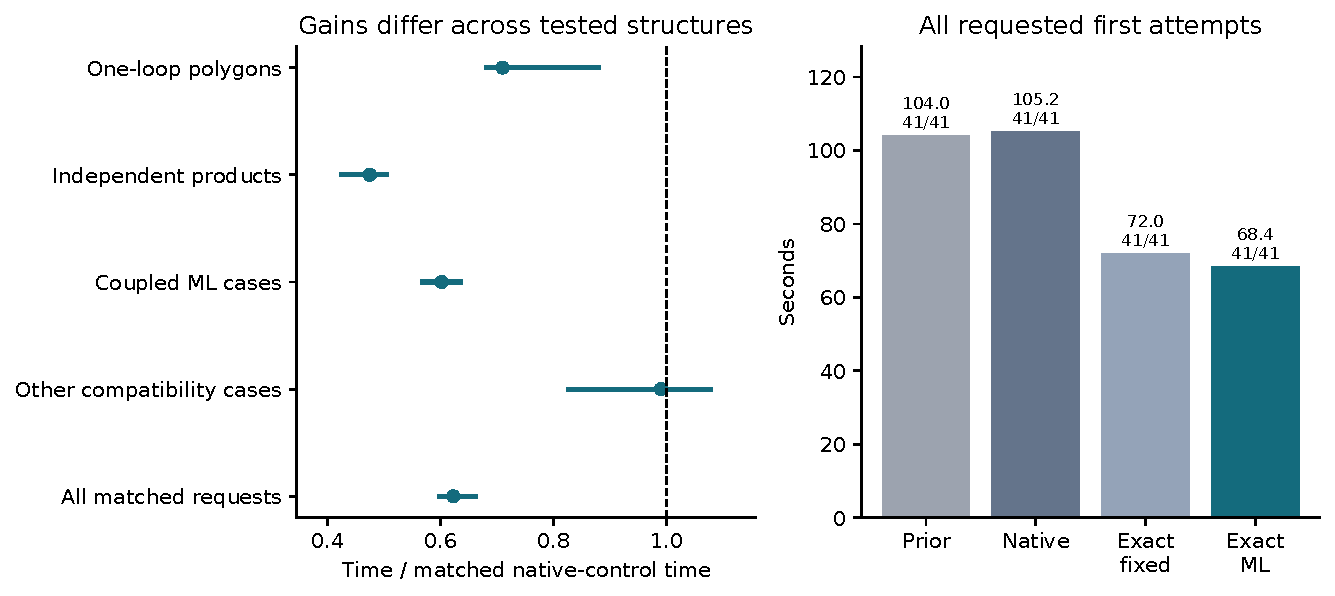
\includegraphics[width=\linewidth]{paper_figures/analytic_decomposition.pdf}
\caption{The left panel compares complete verified reductions with the matched native control. The right panel includes every first attempt and gives completed-request counts above the bars. Intervals describe resampling of three timing repetitions on these fixed requests; they do not establish transfer to every integral family.}
\label{fig:notes-analytic-decomposition}
\end{figure}

The analytic improvement comes from the derived recurrence and shared exact subproblems. The models retain their earlier weights and supported domain, so this experiment does not represent new model training. Independent products provide exact tests through thirteen loops, but their connected components remain one-loop integrals. The separate compatibility cases preserve connected native tests through three loops and the existing thirteen-loop vacuum formula. These measurements do not establish a general analytic solution or a universal speedup for connected high-loop scattering.

The two fully symbolic requests expose a cost hidden by the collection average: their analytic-enabled medians are 1.59 and 3.52 times the matched native medians. Each fresh process loads and uses symbolic algebra before it returns the recurrence result. These measurements compare full paths and do not isolate import time. Section~\ref{sec:notes-parser-guard} tests a separate deployment rule that avoids this setup. The original 41-request measurements remain unchanged.
